
\chapter{Exercise 3}
\label{cha:ugeopgave-3}

In this assignment, I complete every task given in exercise, including the bonus part. The resulting program has the abilities that are expected to perform in Part 1, Part 2 and Part 4 (bonus). The report includes some screenshots of implemented functionalities. For further details, please execute the program itself. 


\section{Part 1}

You can see the screenshots of different blending levels in Figure \ref{fig:3-1}.

\begin{figure}
        \centering
        \begin{subfigure}[b]{0.3\textwidth}
                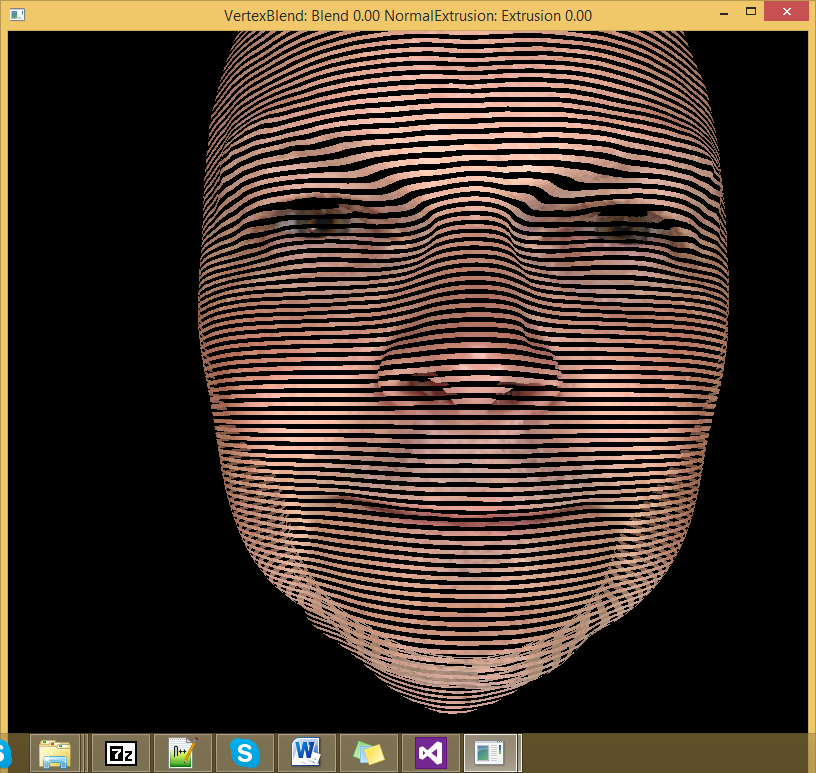
\includegraphics[width=6cm]{../Screenshots/ex-3/1-1.png}
                \caption{Blend Ratio: 0.0}
                \label{fig:3-1-1}
        \end{subfigure}
        
        \begin{subfigure}[b]{0.3\textwidth}
                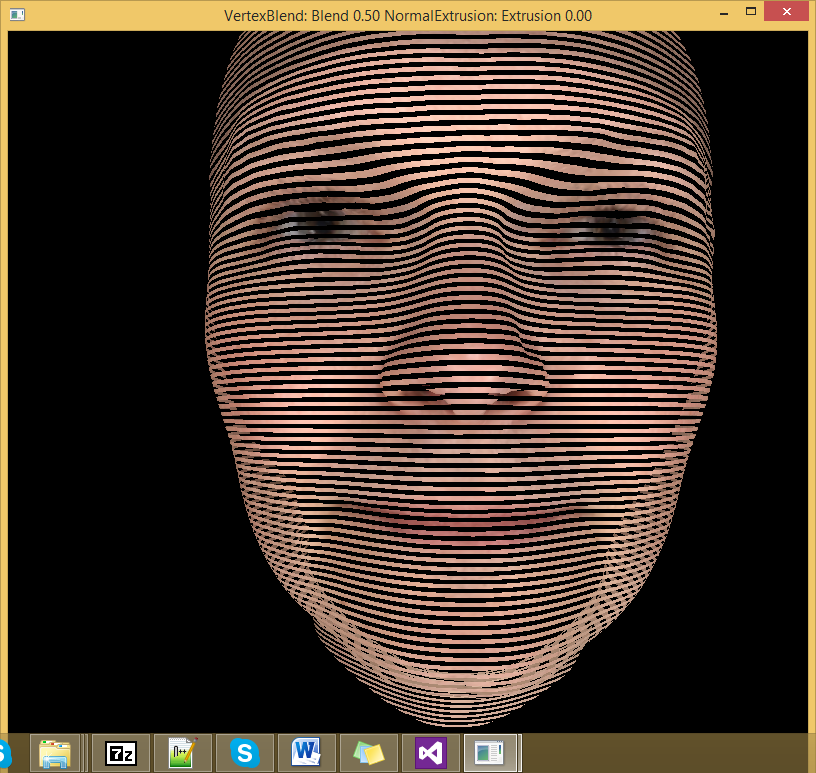
\includegraphics[width=6cm]{../Screenshots/ex-3/1-2.png}
                \caption{Blend Ratio: 0.5}
                \label{fig:3-1-2}
        \end{subfigure}
        
        \begin{subfigure}[b]{0.3\textwidth}
                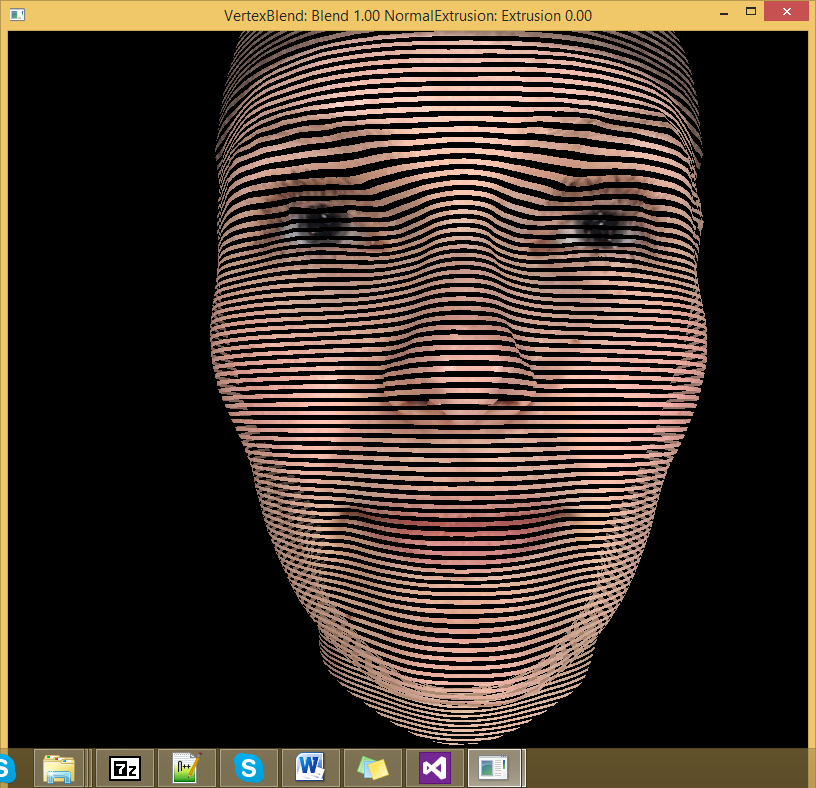
\includegraphics[width=6cm]{../Screenshots/ex-3/1-3.png}
                \caption{Blend Ratio: 1.0}
                \label{fig:3-1-3}
        \end{subfigure}
        \caption{Different Blend Ratios}\label{fig:3-1}
\end{figure}



\section{Part 2}

You can see the screenshots of different normal extrusion levels in Figure \ref{fig:3-2}.

\begin{figure}
        \centering
        \begin{subfigure}[b]{0.3\textwidth}
                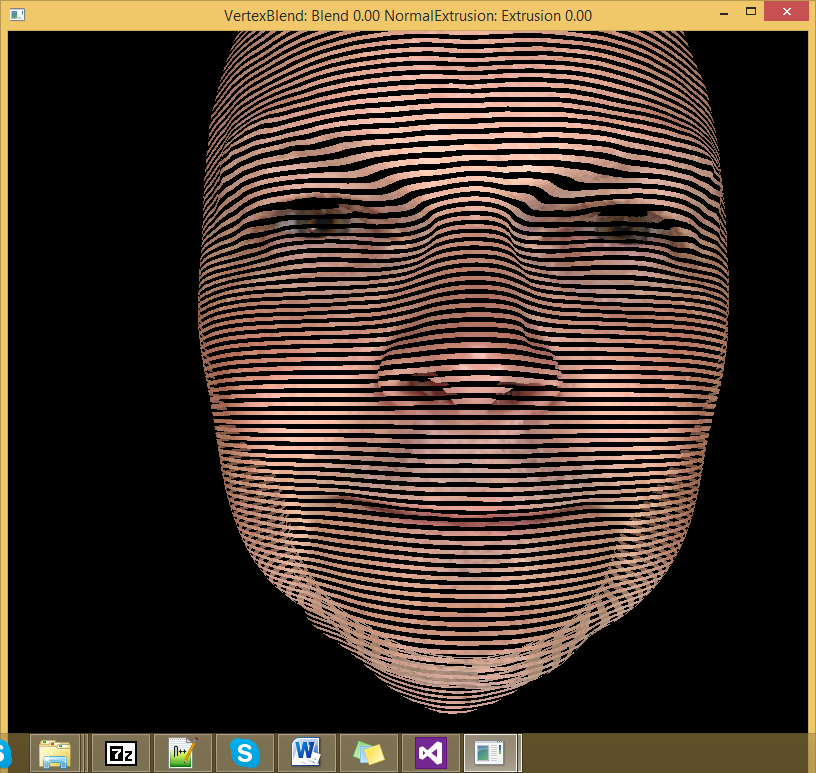
\includegraphics[width=6cm]{../Screenshots/ex-3/2-1.png}
                \caption{Normal Extrusion: 0.0}
                \label{fig:3-2-1}
        \end{subfigure}

        \begin{subfigure}[b]{0.3\textwidth}
                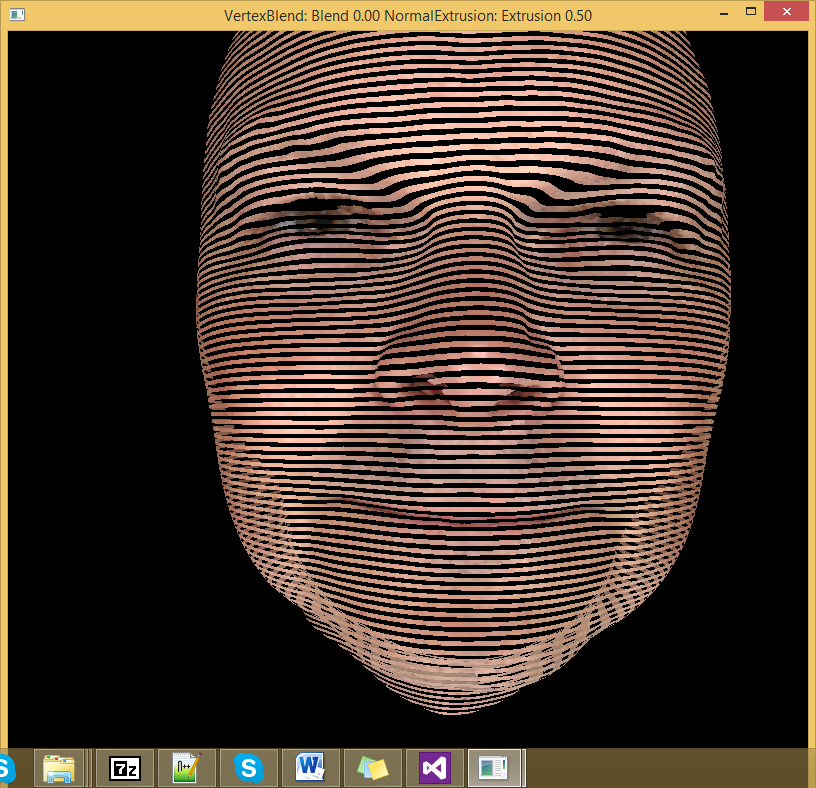
\includegraphics[width=6cm]{../Screenshots/ex-3/2-2.png}
                \caption{Normal Extrusion: 0.5}
                \label{fig:3-2-2}
        \end{subfigure}

        \begin{subfigure}[b]{0.3\textwidth}
                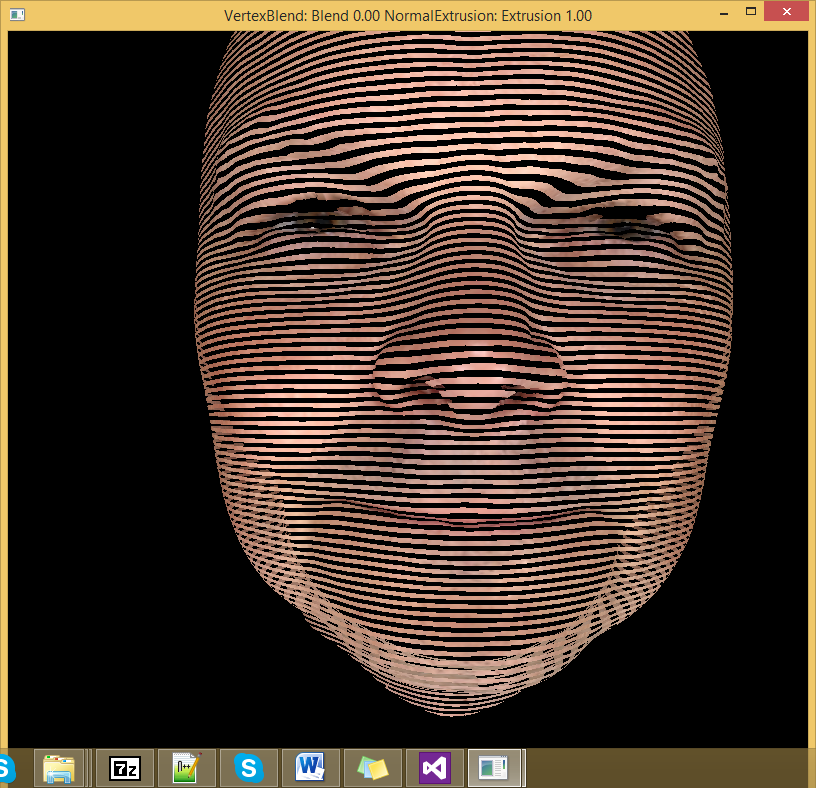
\includegraphics[width=6cm]{../Screenshots/ex-3/2-3.png}
                \caption{Normal Extrusion: 1.0}
                \label{fig:3-2-3}
        \end{subfigure}
        \caption{Different Normal Extrusions}\label{fig:3-2}
\end{figure}



\section{Part 3}

I merge answers of the second, third, and fourth questions and give a mega answer.

\begin{itemize}
  \item Vertex attributes are specific to that vertex: each attribute might differentiate from others.
Unlike vertex attributes, uniform vertex variables are the same for each vertex in model. They can be changed in any callback function.

  \item A vertex shader will transform the representation of a vertex location from whatever coordinate system in which it is
speci?ed to a representation in clip coordinates for the rasterizer .Each invocation of the vertex shader outputs a vertex
that then goes through primitive assembly and clipping before reaching the rasterizer. The rasterizer outputs fragments
for each primitive inside the clipping volume. Each fragment invokes an execution of the fragment shader. Fragment
shader assigns colors to fragments.

  \item Yes it is possible. We need to output two color vectors from vertex shader: color1 and color2. By using uniform \emph{blendingValue}
we can blend two colors in fragment shader. Texturing is applied in fragment shader generally. This is because blending in
fragment shader sounds more natural.
\end{itemize}

\section{Part 4}

As you see in the Figures \ref{fig:3-1} and \ref{fig:3-2}, I make the discard operation successfully. The two lines of code that write in fragment shader is \\

\lstset{language=C}
\begin{lstlisting}
	if(mod(round(glPosition[1]),2.0)==0)
		discard;
\end{lstlisting}


